\documentclass[conference, a4paper]{IEEEtran}
\usepackage{blindtext, graphicx, url}
\hyphenation{}


 %%% JS %%%
%Define the listing package
\usepackage{listings} %code highlighter
\usepackage{color} %use color
\definecolor{mygreen}{rgb}{0,0.6,0}
\definecolor{mygray}{rgb}{0.5,0.5,0.5}
\definecolor{mymauve}{rgb}{0.58,0,0.82}

%Customize a bit the look
\lstset{ %
backgroundcolor=\color{white}, % choose the background color; you must add \usepackage{color} or \usepackage{xcolor}
basicstyle=\footnotesize, % the size of the fonts that are used for the code
breakatwhitespace=false, % sets if automatic breaks should only happen at whitespace
breaklines=true, % sets automatic line breaking
captionpos=b, % sets the caption-position to bottom
commentstyle=\color{mygreen}, % comment style
deletekeywords={...}, % if you want to delete keywords from the given language
escapeinside={\%*}{*)}, % if you want to add LaTeX within your code
extendedchars=true, % lets you use non-ASCII characters; for 8-bits encodings only, does not work with UTF-8
frame=single, % adds a frame around the code
keepspaces=true, % keeps spaces in text, useful for keeping indentation of code (possibly needs columns=flexible)
keywordstyle=\color{blue}, % keyword style
% language=Octave, % the language of the code
morekeywords={*,...}, % if you want to add more keywords to the set
rulecolor=\color{black}, % if not set, the frame-color may be changed on line-breaks within not-black text (e.g. comments (green here))
showspaces=false, % show spaces everywhere adding particular underscores; it overrides 'showstringspaces'
showstringspaces=false, % underline spaces within strings only
showtabs=false, % show tabs within strings adding particular underscores
% stepnumber=1, % the step between two line-numbers. If it's 1, each line will be numbered
stringstyle=\color{mymauve}, % string literal style
tabsize=2, % sets default tabsize to 2 spaces
title=\lstname % show the filename of files included with \lstinputlisting; also try caption instead of title
}
%END of listing package%

\definecolor{darkgray}{rgb}{.4,.4,.4}
\definecolor{purple}{rgb}{0.65, 0.12, 0.82}

%define Javascript language
\lstdefinelanguage{JavaScript}{
keywords={typeof, new, catch, function, return, null, catch, switch, var, if, in, while, do, else, case, break, for},
keywordstyle=\color{blue}\bfseries,
ndkeywords={class, export, boolean, throw, implements, import, this, true, false, Math},
ndkeywordstyle=\color{darkgray}\bfseries,
identifierstyle=\color{black},
sensitive=false,
comment=[l]{//},
morecomment=[s]{/*}{*/},
commentstyle=\color{purple}\ttfamily,
stringstyle=\color{red}\ttfamily,
morestring=[b]',
morestring=[b]"
}

\lstset{
language=JavaScript,
extendedchars=true,
basicstyle=\ttfamily,
showstringspaces=false,
showspaces=false,
tabsize=2,
breaklines=true,
showtabs=false,
captionpos=b
}

 %%% END JS %%%


\begin{document}
\title{How does the implementation of\\
Strategy Design pattern in JavaScript\\
affect Maintainability as measured by Cyclomatic complexity and Lines of code}
\author{\IEEEauthorblockN{Oskar Ther\'{e}n}
\IEEEauthorblockA{Computer Engineering\\
The Institute of Technology at Link\"{o}ping University\\
Email: oskth878@student.liu.se}}

\maketitle

\begin{abstract}
	 In this paper an implementation of the Strategy Design pattern, as described in the book Design Patterns: Elements of Reusable Object-Oriented Software, is presented in the high-level and untyped programming language JavaScript. It is implemented in an existing game, where it replaces a switch statement to reduce cyclomatic complexity. The difference in cyclomatic complexity and lines of code before and after the implementation is evaluated in the aspect of how it affects maintainability. This paper is concluded with some discussion about the usefulness of implementing the pattern in a bigger project.
\end{abstract}

\section{Introduction}
\label{sec:Introduction}
It is widely acknowledged among object-oriented programmers that Design patterns can be useful to solve commonly occurring problems within a given context  by creating reusable code. Design patterns was mainly introduced to software developers through the GoF (Gang of Four) that wrote about the concept in their book, Design Patterns: Elements of Reusable Object-Oriented Software~\cite{bibitem:GoF}, though the idea originally comes from an architectural concept. The patterns has since been widely discussed, customized and used.

% TODO: ADD MORE BELOW
Even though they are so popular there are few empirically justified reasons to use them according to C. Zhang and D. Budgen in their article ``What Do We Know about the Effectiveness of Software Design Patterns?''~\cite{bibitem:Zhang}.

The Design patterns are created from an object oriented perspective, while on the other hand web development is most commonly conducted in the dynamic, untyped and interpreted language JavaScript. JavaScript is often criticized by developers that are used to strongly typed languages, claiming that its static type-checking can lead to unsafe code. A solution to this, proposed by Harmes et al.~\cite{bibitem:DiazHarmes}, is to adapt the GoFs Design patterns to make them applicable to JavaScript, in an attempt to make the code both safer and more reusable.

The purpose of this paper is to find out if the implementation of a specific Design pattern, Strategy [Section~\ref{sec:Strategy}], will affect maintainability [Section~\ref{sec:Maintainability}] in a positive way in the programming language JavaScript.

\subsection{Research Question}
\begin{itemize}
	\item How does the implementation of Strategy Design pattern in JavaScript affect Maintainability as measured by Cyclomatic complexity and Lines of code
\end{itemize}

\subsection{Strategy Design pattern}
\label{sec:Strategy}

An UML-diagram of the concept is shown in [Figure \ref{fig:Strategy}].

\begin{figure}[ht!]
	\centering
	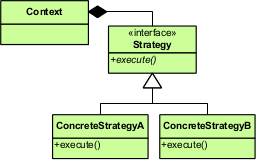
\includegraphics[scale=0.7]{Strategy_Pattern_in_UML.png}
	\caption{Strategy pattern in a UML-diagram}
	\label{fig:Strategy}
\end{figure}

Strategy is a behavioral pattern that intends to minimize coupling by encapsulating a family of algorithms and make them interchangeable by abstracting away the algorithms different functionalities into separate classes that implements a common interface, which is called strategy. For a language to be able to implement Strategy in the way it is explained by the GoF it needs something similar to an Java interface. This does not JavaScript have, which is further discussed in [Section~\ref{sec:JavaScript}].~\cite{bibitem:GoF}

The GoF claims that one of the applications of the pattern is when ``a class defines many behaviors, and these appear as multiple conditional statements in its operations. Instead of many conditionals, move related conditional branches into their own Strategy class''~\cite{bibitem:GoF}. Which gives motivation to why the example [Listing~\ref{lst:switch-case}] in this paper is a good starting point.

\subsection{SOLID}
The purpose of many Design patterns is to solve some of the SOLID-violations that can arise when working on bigger projects. SOLID is an mnemonic acronym that stands for
\begin{itemize}
    \item \emph{Single responsibility} \\
    Each class should only have responsibility over one part of the softwares functionality.
    \item \emph{Open-closed} \\
    Classes, functions and so on, should be open for extension but closed for modification.
    \item \emph{Liskov substitution} \\
    Every subtype should be able to replace its inherited type.
    \item \emph{Interface segregation} \\
    Clients should not be forced to implement methods from and interface that it will not use.
    \item \emph{Dependency inversion} \\
    High level modules should not be affected by changes of low level modules.
\end{itemize}

These principles were developed by RC Martin in his books about Agile development but they can be applicable to a lot of different software development. They are generally good to follow when developing software and are all contributing to code that is for example easier to maintain.~\cite{bibitem:Bob}

The Strategy pattern mainly improves the code with Single responsibility and Open-closed in aspect, although it follows the other principles as well.

\textit{Single Responsibility} through having the code for the algorithms in separate classes.

\textit{Open-closed} because when a new algorithm is introduced, the existing code will not have to be changed. Though a new class for that algorithm needs to be added so the interface is extended.

\subsection{Maintainability}
\label{sec:Maintainability}
The total cost of maintenance in software development is widely discussed and different eminent names in software development have claimed that it will take up from 40 even up to 60 percent of the time and cost to maintain a project. In the 1990s it was claimed by two experts, Corbi and Yourdon, that software maintainability where going to be one of the major challenges for the 1990s. During the 90s this was confirmed by Hewlett-Packard that claimed that ``they had between 40 and 50 million lines of code under maintenance and that 60 to 80 percent of research and development personnel are involved in maintenance activities''~\cite{bibitem:MetricsToEvaluate}.

\subsection{Metrics}

Since the 1991s when the ISO standard for maintainability was introduced (ISO 9126) there have been several attempts to link maintainability with different metrics. Heitlager et al. argues that the problem when the standard was introduced is that ``In general, the proposed metrics for assessing the maintainability characteristics are not measured on the subject of maintenance, i.e. the system’s source code and documentation, but on the performance of the maintenance activity by the technical staff.''~\cite{bibitem:Maintainability}

There are several metrics that tries to measure the complexity of a function or a program. These metrics have different advancement levels, they range from easily measured metrics like just lines of code or cyclomatic complexity to Robillards interconnectivity metric that ``integrates the structural as well as the textual aspects of a program in such a way that the organization of a program can be seen graphically. The measure of complexity depends on how a statement is related to the rest of the program''~\cite{bibitem:Robillard}.

In the article Using Metrics to Evaluate Software System Maintainability Coleman et al. found that when they conducted automated software maintainability analysis on 11 software systems. They all corresponded to the experts intuition and also provided additional useful data. The metric they created is widely used and called MI (Maintainability Index) which is calculated as a factored formula consisting of Source Lines Of Code, Cyclomatic Complexity, Halstead volume and percent of lines of Comments.~\cite{bibitem:MetricsToEvaluate}

Heitlage et al. discusses several problems with MI they are summarized below:
\begin{itemize}
    \item \emph{Root-cause analysis} \\
    Since the formula just gives a number it can be hard to know what the cause of a bad value is.
    \item \emph{Average complexity} \\
    The value will be small even though some functions might have high complexity, since most will not. They argue that an average value is misleading.
    \item \emph{Computability} \\
		The Halstead Volume is difficult to define and compute.
    \item \emph{Comment} \\
		Comments have no correlation with maintainability at all in general.
    \item \emph{Understandability} \\
		The formula is hard to understand since it for example contains several constants that comes without any logical arguments.
		\item \emph{Control} \\
		The developers and management can easily feel a lack of control over the MI value.
\end{itemize}
They moves on to suggest a metric of their own, though it is a bit more complex to go in depth on here. What is important for this paper is that they are also using Lines of Code and Cyclomatic Complexity in their analysis. Though they argues that it is better to calculate Cyclomatic Complexity per unit, where a unit is the smallest piece of code that can be executed and tested individually. Eg. a method in Java.~\cite{bibitem:Maintainability}

\section{Method}
This section presents the JavaScript implementation of the Strategy pattern as well as the chosen metric to evaluate the solution.

\subsection{Interpretation of the Strategy pattern for JavaScript}
\label{sec:JavaScript}
Since JavaScript is not an object oriented language the concept of interface does not exist. In Harmes et al. book ``Pro JavaScript\texttrademark~Design Patterns''~\cite{bibitem:DiazHarmes} the recommendation is to create a Duck Typed interface emulation. This would be useful if the Strategy pattern where used in a real life program to ensure correct parameters where sent to the functions. But since this papers purpose is to evaluate Strategy pattern and uses a quite small example and JavaScript is additionally untyped, the implementation of an interface is skipped and type correctness is assumed.

The example used in this paper is taken from an existing game. The code that is supposed to be replaced with the Strategy pattern is a switch case that sets a \texttt{message} dependent on a string. It is part of a method that renders a message in the \texttt{MainUI} from the method parameter \texttt{entity}, see [Listing~\ref{lst:switch-case}].

The switch case is a violation of the Open/closed principle the goal is to replace it with the calls in [Listing~\ref{lst:strategy}]. This is similar to how the call would look like in the object oriented language Java, a difference is that since JavaScript is untyped everything instantiated with \texttt{var}. The property \texttt{messageType} is replaced with what a more appropriate name \texttt{messageStrategy} and shall be a reference to the correct function instead of a string, e.g.

\begin{lstlisting}[language=JavaScript]
// New
entity.messageStrategy = new humanStrategy();
// Old
entity.messageType = "HumanMessage";
\end{lstlisting}

The Strategy pattern will be implemented in a separate file called \texttt{Messager.js}. It contains a prototype \texttt{Messager(strategy)} that takes a strategy and saves it to its own context \texttt{this}. It also contains a method \texttt{getMessage(...)} that calls the method \texttt{getMessage(...)} on the strategy bound to the context of \texttt{Messager}. The different strategies are in this case also placed in the file \texttt{Messager.js}, so when a new one is needed is just needs to be added to this file. For the resulting file see [Listing~\ref{lst:result}].

\subsection{Metrics}
The chosen metrics for this paper are cyclomatic complexity and lines of code, they are quite easy to measure and is applicable to many languages. Many maintainability metrics use a combination of these metrics in addition of some more.

\subsubsection{Cyclomatic complexity}
It was first developed by Thomas J. McCabe in his ``A Complexity Measure''~\cite{bibitem:CC}. For this smaller example it can be summarized to how many paths a program has where each switch case and if statement creates a new path.

\subsubsection{Lines of code}
This metric can be used to predict maintainability of code, in general the amount of lines of code correlate with how maintainable the source code is. In this paper physical lines of code is used, that counts every line that is not whitespace or comment.

\section{Result}
The result of the two metrics are presented in the subsections below.

\subsection{Cyclomatic complexity}
The cyclomatic complexity of the original code is three, one for each case in the switch case.

After the implementation of the Strategy pattern the complexity is reduced down to one.

\subsection{Lines of code}
The number of lines of code in the original code is 18.

After the implementation of the Strategy pattern the total number of lines of code is increased to 29, though \texttt{MainUI.js} is reduced down to 5 lines.

\section{Discussion}
The result and method is discussed in the following subsections.

\subsection{Result}
The cyclomatic complexity was completely removed from the method \texttt{showMessage} which was the expected result comparing with code examples found at two websites, though they were in the object oriented languages.

One example is by Gil Fink, that has among other co-authored several Microsoft Official Courses. He writes in a blog post about ``Applying Strategy Pattern Instead of Using Switch Statements'' where he applies the Strategy pattern to C++.~\cite{bibitem:GilFink}

Another example though from an unknown source, but. It is a similar implementation of the Strategy pattern made in C\#.~\cite{bibitem:CSharp}

Lines of code had an increase which is to be expected. This can have a negative impact on maintainability, but since the increase of lines is in a new file this does in fact make the \texttt{MainUI.js} more maintainable and less coupled.

When the metrics are combined some conclusions can be drawn:
\begin{itemize}
	\item No matter how big the switch case is \texttt{MainUI.js} will always have the same length with strategy and cyclomatic complexity will be reduced down to one.
	\item The total amount of line of code will increase with two for each switch case that is removed.
\end{itemize}

\subsection{Method}
The implementation of the pattern was not trivial to translate. Since JavaScript is untyped and does not have inheritance this implementation might seem a bit strange for some one not used to Design patterns and object oriented languages. Though if the project is done in object oriented inspired Design, this implementation is quite similar to the e.g. Java version, but then either some version of inheritance should be implemented or at least some check in \texttt{Messager.js} or in \texttt{showMessage()} to handle errors or a default behavior.

The metrics used are the two of the components that Visual Studio by Microsoft uses~\cite{bibitem:MI}. The conclusions drawn from this paper are that they seem to work equally well in JavaScript compared to object oriented languages.

\section{Conclusion}
The definition of the Strategy pattern from the GoF is in some ways lost when translated into JavaScript. Interfaces does not exist and since it is untyped there would be no purpose using inheritance for this pattern. Though if the strategy pattern would be used reoccurring in a project the Duck Typed interface implementation by Harmes et al. is recommended to gain robuster code.~\cite{bibitem:DiazHarmes}

The SOLID principles can be beneficial to implement in JavaScript if the project tries to do a object oriented inspired Design. Design pattern such as Strategy pattern can be implemented quite similarly as shown in this paper and gain some of the benefits to Single responsibility and Open-closed principals.

Despite the benefits, this paper shows that the implementation can increase total lines of code which may have a maintainability drawback. And in search for a in depth evaluation of the pattern in JavaScript the results where only examples of different implementations in JavaScript and explanations why the pattern is beneficial in general object oriented Design.

\clearpage
\section*{Code}

\begin{lstlisting}[language=JavaScript, label=lst:switch-case, caption=\texttt{MainUI.js} The original switch case.]
// Creates and shows a message dependent on entity.messageType
MainUI.prototype.showMessage = function(entity) {
	var message;
	switch(entity.messageType) {
		case "HumanMessage":
			...
			message = ...
			break;
		case "ZombieMessage":
			...
			message = ...
			break;
		case "MonsterMessage":
			...
			message = ...
			break;
	}
	...
};
\end{lstlisting}

\begin{lstlisting}[language=JavaScript, label=lst:strategy, caption=\texttt{MainUI.js} Switch case replaced trough the Strategy pattern.]
// Creates and shows a message dependent on entity.messageStategy
MainUI.prototype.showMessage = function(entity) {
	var messager = new Messager(entity.messageStrategy);
	var message = messager.getMessage(...);
	...
};
\end{lstlisting}
\newpage
\begin{lstlisting}[language=JavaScript, label=lst:result, caption=\texttt{Messenger.js} Resultant Strategy code\, strategy function names are the values of \texttt{ObjectTypeEnum}.]
Messager = function(strategy) {
  this.strategy = strategy;
};

Messager.prototype.getMessage = function(...) {
  return this.strategy.getMessage(...);
};

var humanStrategy = function() {
  this.getMessage = function(...) {
    ...
    return message;
  };
};

var zombieStrategy = function() {
	this.getMessage = function(...) {
		...
		return message;
	};
};

var monsterStrategy = function() {
	this.getMessage = function(...) {
		...
		return message;
	};
};
\end{lstlisting}
\newpage
\begin{thebibliography}{1}
\bibitem{bibitem:GoF}
Erich Gamma, Richard Helm, Ralph Johnson and John Vlissides, \emph{Design Patterns: Elements of Reusable Object-Oriented Software} \hskip 1em plus 0.5em minus 0.4em\relax Addison-Wesley Professional, 1st edition, January 15, 1995
\bibitem{bibitem:Zhang}
Cheng Zhang and David Budgen, \emph{What Do We Know about the Effectiveness of Software Design Patterns?} \hskip 1em plus 0.5em minus 0.4em\relax IEEE Transactions on Software Engineering, vol. 38, no. 5, pp. 1213-1231, September-October 2012
\bibitem{bibitem:Bob}
Robert C.~Martin, \emph{Agile software development: principles, patterns, and practices} \hskip 1em plus 0.5em minus 0.4em\relax Agile software development: principles, patterns, and practices, 2002
\bibitem{bibitem:MetricsToEvaluate}
Don Coleman, Dan Ash, Bruce Lowther and Paul Oman, \emph{Using Metrics to Evaluate Software System Maintainability} \hskip 1em plus 0.5em minus 0.4em\relax Computer, Volume:27,  Issue: 8, August 1994
\bibitem{bibitem:Maintainability}
Heitlager, Ilja, Tobias Kuipers, and Joost Visser. \emph{A practical model for measuring maintainability} \hskip 1em plus 0.5em minus 0.4em\relax In Quality of Information and Communications Technology, 2007, pages 30-39
\bibitem{bibitem:Robillard}
Pierre N.~Robillard and Germinal Boloix, \emph{The Interconnectivity Metrics: A New Metric Showing How a Program Is Organized} \hskip 1em plus 0.5em minus 0.4em\relax Journal of Systems and Software, Volume 10, Issue 1, July 1989, Pages 29-39
\bibitem{bibitem:DiazHarmes}
Dustin Diaz and Ross Harmes, \emph{Pro JavaScript design patterns} \hskip 1em plus 0.5em minus 0.4em\relax Apress, 2008
\bibitem{bibitem:GilFink}
Gil Fink, \emph{Applying Strategy Pattern Instead of Using Switch Statements}, \url{http://blogs.microsoft.co.il/gilf/2009/11/22/applying-strategy-pattern-instead-of-using-switch-statements/}, Accessed: 2017-06-07
\bibitem{bibitem:CSharp}
\emph{How to use Strategy Pattern Instead of Switch-Case statements}, \url{https://vcpptips.wordpress.com/tag/cyclomatic-complexity/}, Accessed: 2017-06-07
\bibitem{bibitem:CC}
Thomas J. McCabe, \emph{A Complexity Measure} \hskip 1em plus 0.5em minus 0.4em\relax in IEEE Transactions on Software Engineering, vol. SE-2, no. 4, pp. 308-320, Dec. 1976
\bibitem{bibitem:MI}
Microsoft Developer Network, \emph{Code Metrics Values}, \url{https://msdn.microsoft.com/en-us/library/bb385914.aspx}, Accessed: 2017-06-08
\end{thebibliography}

\section*{Improvements after submission}

\end{document}
